\chapter{Choice Poetics}

\label{ch:choice-poetics}

The aim of this chapter is twofold--first, to establish a framework for talking clearly and precisely about choices and their outcomes, and second, to introduce a method for analyzing choices based on how they relate to player goals.
%
Choice poetics should be able to address questions like: ``What is it about a choice that makes some players feel regret after picking a particular option?''
%
This chapter attempts to establish terminology and formal perspectives that can be used to talk about choices, but it's far from a ``complete'' theory of choice poetics: it only deals with explicit, discrete choices, for example.
%
Some parts of the theory are more developed (those that supported and were influenced by the development of \dunyazad/), but the ideas here are just the beginning of an in-depth study of narrative choices.


\section{Inspirations}

While choice poetics clearly has roots in the work of Aristotle \citep{Aristotle1917} (and more recently narrative formalists like Freytag \citep{Freytag1894} and Barthes \citep{Barthes1975}, to name only a few) choice poetics is also inspired by investigations into the psychology of both reading and decisions.
%
In the first camp, authors like 
% TODO: HERE

\citep{Carr2009}
\citep{Bizzocchi2011}


\section{Modes of Engagement}


In developing a theory of choice poetics, one must respect the lessons of the development of traditional poetics.
%
In particular, modern scholars have largely rejected ``objective'' narrative analysis and concluded that the experience of the individual reader must be taken into account.
%
Unlike Aristotle, who stated authoritatively what was good and bad about this drama or that, modern narrative scholars will analyze a work from a particular perspective, without claiming that this perspective is universal, perhaps performing a feminist or Marxist reading of a novel to see what insights a particular lens has to offer about the work.


Choice poetics must also respect the perspective of the reader, but it is in a slightly different position, as its readers are also players.
%
Insofar as the narrative that contains choices is experienced through the fabric of a game, the reader/players (henceforth players) are stepping into the magic circle of the game \citep{Huizinga1949} and intentionally taking on certain attitudes.
%
A narrative experienced within the framework of a game thus implicitly biases the attitudes of its readers, for example by setting up a score counter which players can try to maximize.
%
Counter-play is of course possible and important, but even counter-play is influenced by the rules of the game by virtue of being set against them.
%
The formal structures of the game rules that accompany a narrative-with-choices thus allow the theoretician to make an educated guess about the attitudes of players interacting with a piece.


There are still a range of attitudes that players can take on, however, and some understanding of this range is important before any analysis of choices in a narrative.
%
This range of attitudes has to some degree been studied by others interested in player types, although such studies are mostly focused on games without regard to narrative.
%
From simple binary ``casual/hardcore'' distinctions to more complex typologies such as Bartle's ``achievers,'' ``explorers,'' ``socializers,'' and ``killers,'' \citep{Bartle1996} player type classifications to some degree incorporate notions of player intent or attitude.
%
However, player type classifications also focus on player actions or approaches within the game, for example a distinction between those who enjoy stealth or direct combat more.
%
These player content preferences are as important as any other player preferences when it comes to how players approach choices, but they're less important than player motivations, which establish entire contexts within which preferences can be expressed.
%
For example, if one's motivation to play is a desire to act out a role, one's preferences might be expressed in terms of the kind of role one is trying to act out.
%
If one's motivation to play is to score points, on the other hand, preferences might be expressed in terms of different strategies for doing so.


The idea of ``modes of engagement'' captures these different player motivations.
%
Modes of engagement are different ways in which a player can approach a game.
%
At this point it is important to note that modes of engagement are neither exclusive nor permanent: players often engage in several modes at once (to varying degrees) and may change their modes of engagement during the course of play.
%
The modes of engagement presented here are also not intended to be comprehensive: these are some of the most common modes, but others may be possible and even the norm for certain games.
%
All of that notwithstanding, consideration of the mode(s) of engagement that players bring to a work is the first step in analyzing the choice poetics of a work.


This can take the form of assuming a particular mode: much as one can perform a feminist reading of a novel, one could perform a power-playing playthrough of a game.
%
This could also take the form of analyzing the game itself to determine which mode(s) of engagement it encourages and rewards.
%
It could even take the form of a qualitative study of actual players, to determine which mode(s) of engagement they are employing.
%
In any case, an analysis of choice poetics that does not consider modes of engagement is incomplete.


\Cref{tab:modes-of-engagement} lists some of the most common modes of engagement, and gives examples of decisions that employ them.
%
The last column references Nick Yee's work on motivations for play in massively-multiplayer online role-playing games as a comparison \citep{Yee2006}.
%
The grouping of Yee's motivation components into these modes of engagement has to do with a difference in focus: Yee is focused primarily on aspects of play, including a strong focus on online social interaction, whereas choice poetics is interested primarily in single-player offline engagement with an emphasis on narrative.
%
For example, Yee makes fine distinctions between different motivations grouped into the ``power play'' category here, but from a choice poetics perspective, whether someone is trying to maximize score or compete with an opponent doesn't matter, because both motivations are equally orthogonal to the narrative, and thus they have a similar effect on the player's experience of the narrative.


\begin{table}[h]
\begingroup
\renewcommand*{\arraystretch}{1.5}
\begin{tabular}{p{5em}p{10em}p{10em}p{7em}}
\textbf{Mode} & \textbf{Decision Process} & \textbf{Example} & \textbf{\citep{Yee2006}} \\
\hline
\textbf{Avatar Play} & Decide as if you were in the character's situation. & When picking a pet, pick the cat because you like cats. & Role-Playing, Customization, Escapism \\
\textbf{Role Play} & Decide in order to act out a persona. & Choose the wizard character class because you want to play a shy, bookish person. & Role-Playing, Customization, Escapism \\
\textbf{Power Play} & Choose options that advance game metrics like score, beating other players, or quick completion. & Sacrifice an ally to obtain a powerful item because it helps you beat the game more quickly. & Advancement, Mechanics, Competition, Teamwork \\
\textbf{Explora-tory Play} & Choose options to see what will happen. & Turn away from the path of your quest to explore the world. & Discovery \\
\textbf{Social Play} & In a multiplayer situation, choose options because of social considerations. & Turn down a high-level quest in order to accompany your friend on a lower-level quest. & Socializing, \newline Relationship \\
\textbf{Analyti-cal Play} & Make decisions in order to analyze the work. & Repeatedly load a saved game to explore every possibility at a choice. & \emph{none} \\
\textbf{Critical Play} & Make decisions as performance to deconstruct or criticize a work. & Drive your character into poverty in order to demonstrate a game's biased depiction of poor people. & \emph{none} \\
\end{tabular}
\endgroup
\caption[Modes of engagement]{Some common modes of engagement.}
\label{tab:modes-of-engagement}
\end{table}

Although modes of engagement are important to choice poetics, in my work with \dunyazad/ I have not given them great attention: \dunyazad/ encourages avatar play and all of its evaluations assume that players will engage primarily in this mode.
%
Extending \dunyazad/ to support power play and role play better, and to account for these possible approaches when evaluating choices, would be a very interesting line of future work.
%
Developing \dunyazad/ in that direction would allow it to be used as a tool to study modes of engagement in more detail.


\section{Dimensions of Player Experience}

When using choice poetics to analyze a narrative or even just a single choice, one must consider the range of expressiveness of narrative choices.
%
Aristotle devoted much of his analysis in \work{Poetics} to comedy and tragedy as two of the most important modes of drama in his day, but the full range of poetic effects is very broad, and includes both momentary impressions such as a single confusing sentence and overall feelings, such as a vague dissatisfaction with an entire novel.
%
Once choices are involved, this repertoire is expanded, and it's important to have some understanding of what poetic effects a choice can possibly have.
%
Although no summary of possible poetic effects could hope to be complete, I have tried to list here a collection of important high-level aspects of a narrative experience that are strongly influenced by choice structures, including some which I believe are unique to narratives that contain choices.


\begin{table}[h]
\begingroup
\renewcommand*{\arraystretch}{1.5}
\begin{tabular}{p{5.5em}p{14em}p{13em}}
\textbf{Dimension} & \textbf{Description} & \textbf{Supported By} \\
\hline
\textbf{Absorption} & How much of the player's attention is focused on the game. & Outcomes that are believable given options. \\
\textbf{Identifica-tion} & How comfortable the player feels in the role they play as their avatar. & Options that support player self-expression. \\
\textbf{Transpor-tation} & The degree to which a player thinks in terms of the game world rather than the real world. & Choices where the available options cover what the player thinks should be possible. \\
\textbf{Agency} & Alignment of player goals with game affordances. & Transparent choices where outcomes align with player goals.\\
\textbf{Influence} & Degree of player control over in-game outcomes. & Choices where outcomes are divergent and impactful. \\
\textbf{Autonomy} & The player's ability to choose and pursue a variety of goals at their own discretion. & Choices between goals rather than between methods of pursuing a fixed goal; non-exclusive outcomes. \\
\textbf{Responsi-bility} & Player feelings of responsibility for the actions of their avatar. & A mix of intentional outcomes that are good for and bad for other game characters. \\
\textbf{Regret} & Player feelings of regret for an in-game decision. & Negative outcomes that result from tempting options but which are still believable. \\
\end{tabular}
\endgroup
\caption[Dimensions of player experience]{Some aspects of player experience that are influenced by choice poetics.}
\label{tab:dimensions-of-experience}
\end{table}

\Cref{tab:dimensions-of-experience} provides a brief overview of these important dimensions of player experience.
%
Except for identification, transportation, and absorption, each of these possible poetic qualities are unique to interactive narratives: without choices, they simply aren't possible.
%
Because of this, figuring out how choice structures contribute to these effects 
is an important task for choice poetics.
%
Of course, some of these effects, like agency, have already been extensively studied, often in broader contexts than just choice-based interactive narrative.
%
But it will still be important to understand how choice structures specifically contribute to these poetic qualities.
%
What follows is a preliminary analysis of each quality, based on craft wisdom and existing studies of games and real-world choices.

\begin{itemize}
  \item \textbf{Absorption} -- The idea of `immersion' is often discussed in relation to games, but the concept is often unclear, as it can refer to anything from immersion in an imagined world to sensory immersion in a virtual reality experience.
%
Absorption simply refers to the player's division of attention--is the player's attention completely absorbed by the narrative experience (whether it's a book, live-action role-playing game, or headset-enabled virtual reality experience) or are they distracted from the narrative?
%
Although considering this as a poetic quality is counter-intuitive, it's actually possible for a narrative to distract the player from itself by raising outside issues or causing emotions like frustration.
%
This is particularly relevant when choices become involved, as they can easily become a source of frustration.

  \item \textbf{Identification} -- Identification in traditional narrative is a key property and is heavily influenced by the actions and attitudes of the main character.
%
In narratives that include choices, the player usually has some control over the actions of the main character, although this control is often incomplete, especially when it comes to attitudes rather than actions.
%
Choices can have a big impact on identification if they fail to include options which the player believes are reasonable and which correspond to the choice that the player would be most comfortable with in a given situation.
%
For example, if the player is a pacifist, but there are never options for negotiating with enemies or otherwise resolving conflicts peacefully, one would expect identification to be hindered.
%
This is complicated by role-playing, however: a player who is a pacifist in real life may enjoy the opportunity to play a bloodthirsty character in a game.

  \item \textbf{Transportation} -- Transportation is to some degree linked to identification, as when one identifies with a character it becomes easier to project oneself into that character's world.
%
Again, the believability and completeness of options and outcomes is important when choices come into the picture.
%
Any time that a player begins to think ``I wish I could do X here,'' that player has started to think about the game from an analytical point of view instead of within the game's world.
%
Choices can also encourage transportation by presenting options which require mental effort to assess.
%
When a player starts thinking carefully about the consequences of a particular action within the game world (from a narrative point of view, at least) they are thinking from a perspective that is within that world, which is exactly the phenomenon of transportation.

  \item \textbf{Agency} -- Agency has been a core focus of games studies as a feeling uniquely enabled by interactive media.
%
The feeling of empowerment that results from being able to achieve one's goals contributes to agency, and an alignment of player goals with player-influenced outcomes is a powerful formula for agency.
%
Obviously, such an alignment relates intimately to choice structures, as choice structures establish which outcomes can be influenced by the player and also help set player expectations as to their goals.
%
Given this, opaque choices--where the player is not able to foresee consequences given the setup and options--usually decrease agency, because even if an outcome advances player goals, the player doesn't feel responsible for their success.
%
Additionally, choices where outcomes are tangential to a player's goals can frustrate agency: if you're told to save the princess but then given only choices about which commodities to buy or sell, your ability to proactively pursue your goal has been stifled.

  \item \textbf{Influence} -- Related to agency, but slightly simpler, is the concept of influence: how influential the player feels within the narrative world.
%
Influence can be either \emph{passive} or \emph{active}: passive influence is the ability to affect the success or failure of some important event, whereas active influence is the ability to decide between substantially different plot developments.
%
A game like Final Fantasy \citep{FinalFantasy} gives the player mostly passive influence: the player-controlled characters are hugely influential in the story world, and the player's choices when successful drive that influence, but the player has very few choices that actually decide between different fates for the world, and in fact many key character decisions are taken out of the hands of the player.
%
A game like Sim City \citep{SimCity} provides active influence: the story of the city that the player creates will turn out wildly different depending on the choices the player makes.
%
Of course, Sim City is not usually thought of as a narrative game, and there are fundamental problems with providing active influence in games that have strong stories.

  \item \textbf{Autonomy} -- Autonomy is also related to agency and influence, and can be summarized as the player's ability to choose and pursue their own goals within a game.
%
Some amount of active influence is required to have autonomy, but whereas influence is concerned with outcomes, autonomy is concerned with goals.
%
A game that supports player autonomy provides a play-space within which players can choose their own goals.
%
To the extent that a narrative-focused game can provide this, it will appear more as a space for player-created stories than a fixed story that affords the player some choice.
%
Games like Sim City \citep{SimCity} and The Sims \citep{TheSims} provide play spaces within which players can create their own narratives, and this is achieved by offering non-explicit non-discrete choices which give the player a huge amount of options.
%
A lesser degree of autonomy can be present in more linear narratives when the player has choices which affect the goals and priorities of characters within the story.

  \item \textbf{Responsibility} -- A feeling of responsibility for one's own actions (as distinct from empathizing with a character who feels the burden of responsibility) is something uniquely afforded by interactive narratives.
%
Choice structures are key to creating this, and there are several conditions for enabling responsibility.
%
First, the player must be given moral agency within the story world, which means that different outcomes at a choice must have consequences which have morally different outcomes.
%
Second, the player must be willing to take responsibility for their actions, and this can be impeded when they feel that the outcomes of their actions were unforeseeable or otherwise out of their control (of course, the feeling of a player who mentally justifies their lack of culpability for an in-game consequence is also an interesting poetic effect).
%
Note that this direct player-responsibility is different from role-played responsibility: it's possible for a player to role-play responsibility even when the actions they are assuming responsibility for were completely outside their control.
%
An example of responsibility (or the shirking thereof) as a poetic effect happens in the game Portal \citep{Portal}, when the player is forced to incinerate their companion cube in order to progress within the game.
%
The complex emotions that arise at that moment are the result of a forced choice between two bad outcomes (being unable to progress and incinerating the companion cube\footnote{Note that this analysis makes assumptions about the player's goals and feelings: some player communities see the companion cube itself as an obstacle worthy of hatred rather than a helper who deserves pity, and so view this choice in a very different light.}), and the moment has emotional resonance later in the game when the player has the opportunity to destroy GLaDOS--the agent which forced the decision upon the player.


  \item \textbf{Regret} -- Like responsibility, the capacity to make players feel regret is unique to interactive narrative.
%
Again, in linear narrative it is possible to sympathize and empathize with a character who is feeling regret within the story, but that's a different feeling than personal regret for one's own actions.
%
As with responsibility, making a player feel regret is quite delicate: the player not only has to achieve some level of transportation and identification, but the choices involved must be structured to resist the player's natural tendency to reassign blame.
%
With a negative emotion like regret, the basic psychological mechanisms of denial are the brain's first line of defence, and so naturally the narrative and choices leading up to a moment of regret will be scrutinized for interpretations that leave the player blameless.
%
In particular, if the player can convince themselves that the game forced them to make a choice that led to a negative outcome, or that the outcome was unforeseeable given the option that led to it, they can avoid regret.
%
Of course, this process of denial is an interesting poetic effect in its own right, and in some cases is exactly what an author wants (perhaps so they can later force the player to re-examine their denial and admit blame, thus experiencing even more poignant regret).
%
A game like The Walking Dead \citep{TheWalkingDead} forces the player to make many difficult decisions between options with divergent but uniformly negative consequences, and this pattern engenders feelings of desperation and regret.

\end{itemize}


Each of these topics could be (and some of them have been) the topic of dedicated research.
%
However, they are presented here merely to demonstrate how much there is to learn about choice poetics--\dunyazad/ as a system does not focus on any of these, but rather attempts to get at some simpler phenomena, such as what makes an individual choice obvious, or what is required for a choice to be seen as a dilemma.
%
Patterns of choices with specific properties such as obviousness or unexpectedness of outcomes come together to produce higher-level poetic effects like those described here, and a better understanding of these low-level effects is required in order to aim at these high-level effects.
%
The poetic details that \dunyazad/ actually operationalizes are based on player goals, and the perceived relevance of options and outcomes to them.
%
As \dunyazad/ only reasons about one choice at a time, its logic effectively comprises an analysis technique for examining the basic poetic properties of an individual choice.
%
The next section describes this technique and how a human would apply it to an individual choice within an interactive narrative, while \cref{ch:dunyazad} describes how \dunyazad/ operationalizes this theory, and \cref{ch:results} describes how results from experiments using \dunyazad/ have informed both the theory and the system.

\section{Goal-Based Choice Analysis}

When authoring a choice or attempting to understand an existing choice, the method of analysis presented here can help tease out how a choice might be perceived by players.
%
This method is grounded in player goals: it views each option and outcome through the lens of what the player wants, and then tries to synthesize this information to understand how an entire choice is perceived.
%
\cref{fig:choice-analysis-method} gives an overview of the technique described in this section, which consists of seven steps.
%
The basic idea is to carefully break down how the options and outcomes relate to player goals, attempting to consider as many details as possible, and then synthesize those detailed assessments back into high-level assessments of the choice as a whole.
%
The next section describes in detail how a discrete, explicit choice is represented for this analysis, and the seven analysis steps are described in the sections that follow.

\begin{figure}[h]
\centering
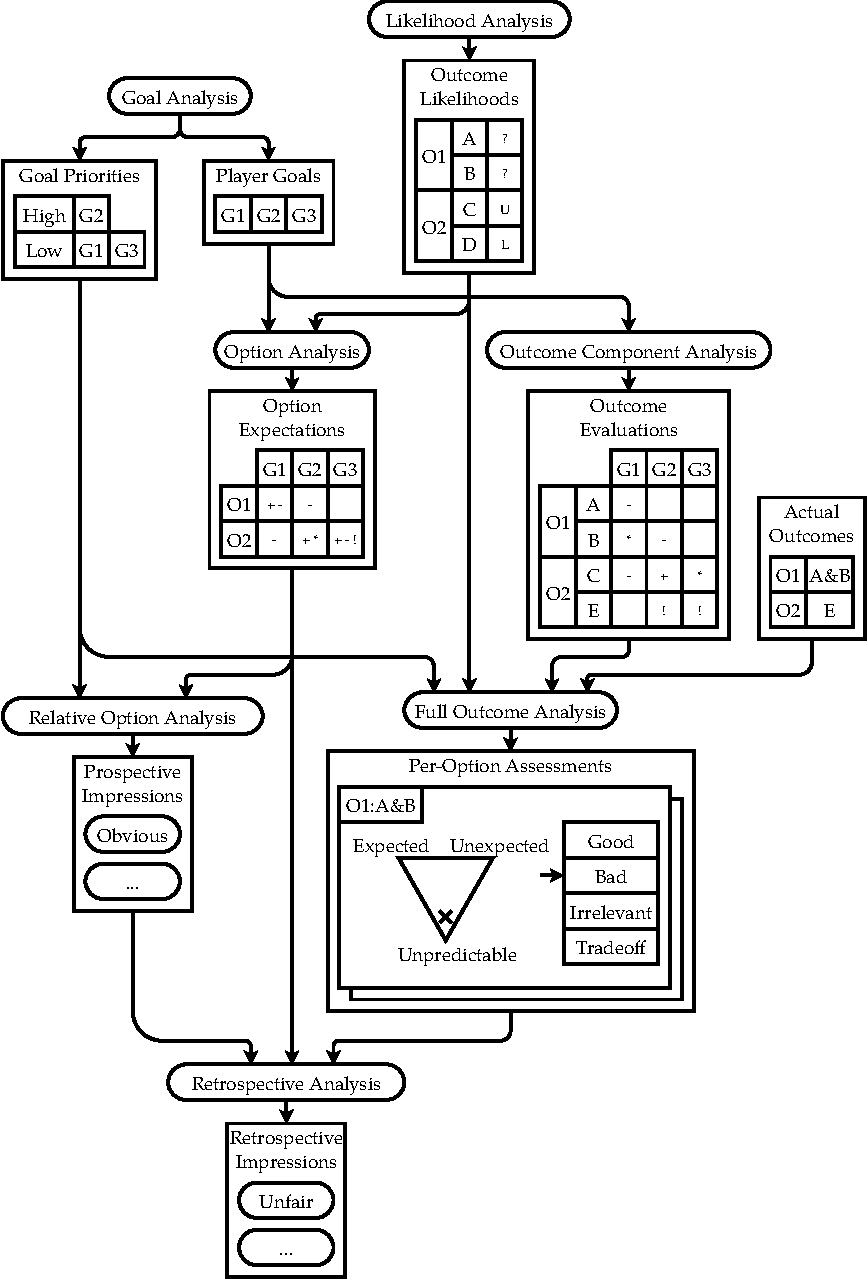
\includegraphics[height=\textheight]{fig/analysis-method-crop.pdf}
\caption[Choice analysis flowchart]{Goal-based choice analysis for a single choice--an overview of the different steps and the information produced.}
\label{fig:choice-analysis-method}
\end{figure}


\subsection{Choice Representation}

This method is developed primarily for the analysis of explicit discrete choices, and for these choices a detailed breakdown of their structure is possible.
%
\Cref{fig:choice-anatomy} shows how a choice (in this case one generated by \dunyazad/) can be broken down into framing, options, and outcomes.
%
Note that it can be useful to further break down the outcomes into individual components: changes that result from an option which are individually significant.
%
By doing so, the impact of each outcome component on individual player goals can be analyzed separately, which helps understand outcomes that involve complex trade-offs between multiple goals.
%
Not shown in \cref{fig:choice-anatomy} are the unrealized outcome components which nevertheless factor into the choice analysis.
%
For example, if the player were unlucky, the third option might not have resulted in the bandits calming down, and one could even imagine a situation where the bandits might turn on the player.
%
Understanding what the player thinks \emph{might} happen as a result of choosing a given option is just as important as recognizing what does happen as the story unfolds.
%
This idea of potential outcome components can also help analyze cases where a system is nondeterministic, and the outcomes of a choice vary between playthroughs.
%
Each part of a choice is subject scrutiny using the methodology presented here, and having precise language to talk about these choice components is necessary for detailed analysis.

\begin{figure}[h]
\centering
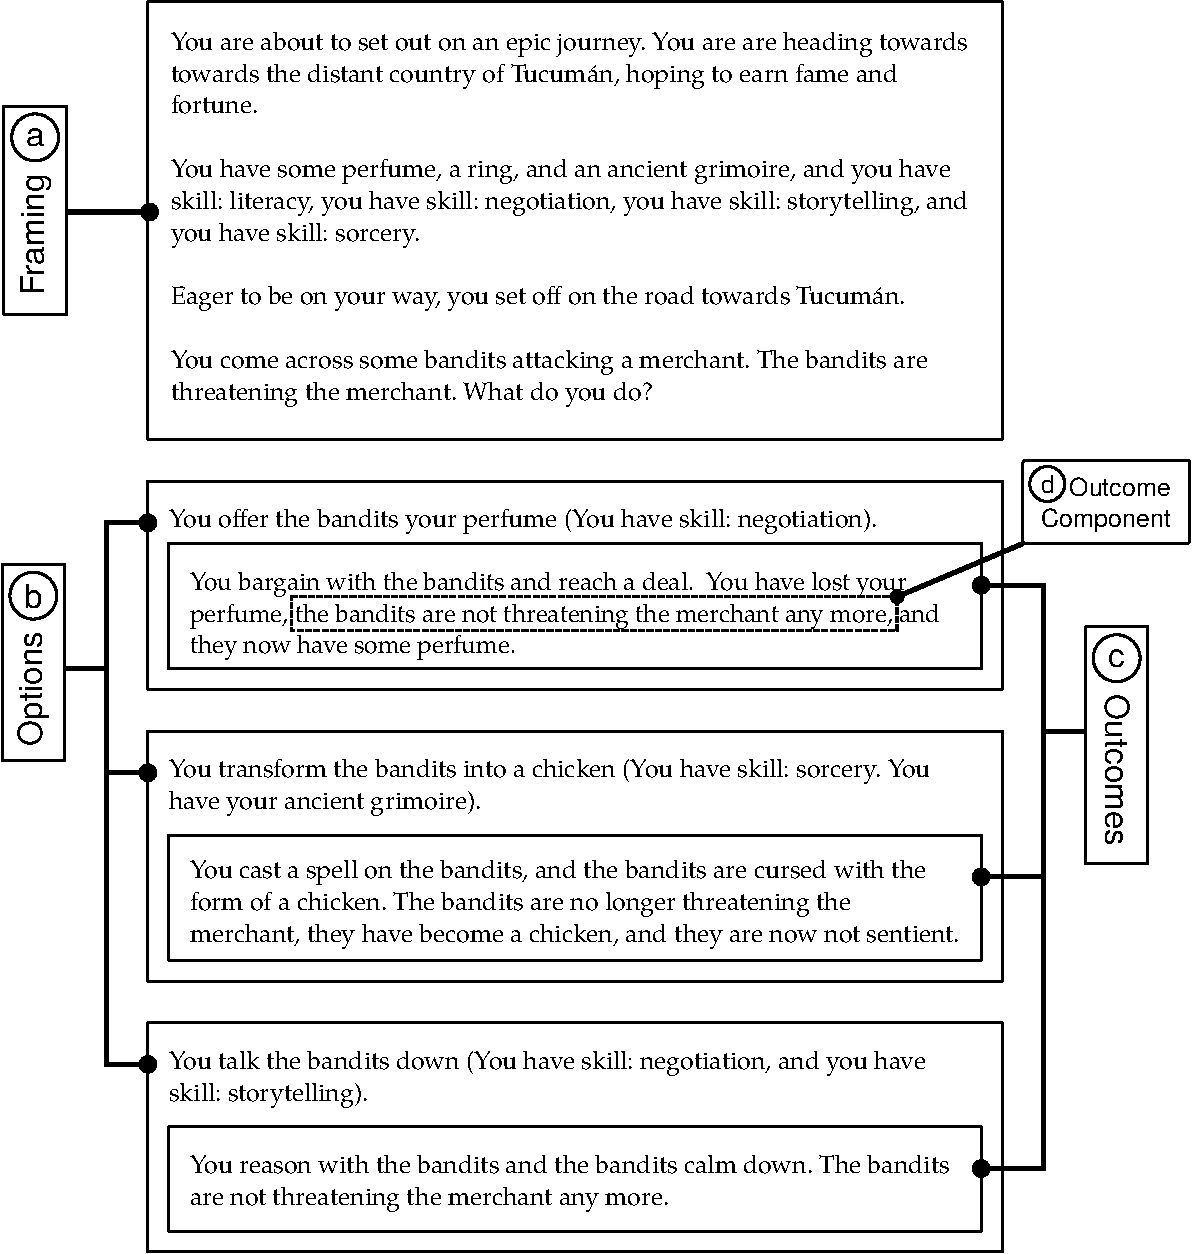
\includegraphics[width=\textwidth]{fig/choice-anatomy-crop.pdf}
\caption[Anatomy of a choice]{%
\setstretch{1.1} % Else the \encircles would stretch only some of the lines
Anatomy of a choice (using one generated by \dunyazad/). \encircle{a}~Framing--sets up the narrative situation at the choice. \encircle{b}~Options--discrete options available to the player. \encircle{c}~Outcomes--Not initially visible to the player, but revealed after a decision is made. Each option has a single corresponding outcome. \encircle{d}~Outcome components--Individually significant changes that result from picking a particular option.}
\label{fig:choice-anatomy}
\end{figure}


\subsection{Goal Analysis}

As already mentioned, poetic analysis of a choice depends on some understanding of the player's approach to the choice.
%
For goal-based choice analysis, this is taken into account by coming up with a list of player goals.
%
Depending on the objective of analysis, there are different ways to come up with this list.
%
One method is to simply list the goals that the analyst themselves would have when approaching the choice.
%
Another is to try to put oneself in the shoes of a particular type of player, perhaps according to one of the modes of engagement listed above.
%
This can be useful for an author trying to figure out how different types of players will perceive a choice: just come up with goal lists corresponding to each player type of interest and perform separate analyses using each list.


In any case, coming up with these lists should take into account not only the desires of the actual or imagined player, but also what aspects of the framing of the choice and previous content encourage which player goals.
%
Based on the options available at previous choices and the narrative content, games can not only encourage certain general modes of engagement, but can establish and encourage the pursuit of specific goals.
%
This encouragement itself often depends on a player's mode of engagement to function as intended, however.
%
For example, game rules directly establish goals for power gamers, but player who have a different mode of engagement may not care about those goals.


If an important goal is missing from the goal list, the entire analysis may be skewed, so it's important to consider the full set of probable player goals.
%
On the other hand, it's always possible to come back to the goal analysis if one realizes during a later step that there's an additional goal that might be relevant. 
%
This is not uncommon, as the particular set of options and outcomes at a choice  determines which goals are relevant.
%
However, part of the point of performing goal analysis before even considering the structure of the choice in question is to avoid bias.
%
This also means that the results of goal analysis can be re-used when analyzing multiple choices.
%
Of course, player goals may change over the course of a game, and this must be taken into account, but performing a full goal analysis from scratch for each individual choice is generally not necessary.


Besides just listing player goals, a goal analysis must give some notion of their relative priorities.
%
This can be as simple as sorting the goals into ``high'' and ``low'' priority tiers, but a more detailed representation of priorities can also be used.
%
This priority information is used when combining information about multiple options and outcomes during the relative option analysis and full outcome analysis steps.
%
Because goal priorities are even more volatile and difficult to estimate than goals themselves, sometimes it's simplest just to wait until the later analysis steps to consider goal priorities, as there will likely be only a few specific goals (those relevant to the choice in question) for which priorities actually affect the analysis.


\subsection{Likelihood Analysis}

The second step of analysis is to figure out which potential outcome components are made to seem likely by the framing and option text of the choice.
%
This step starts by identifying a set of outcome components that seem plausible, and then isolating a subset of those that seem likely.
%
If desired, finer gradations of likelihood can be used, but at least finding a set of plausible outcomes and distinguishing some of those as likely is required.
%
The outcome likelihoods produced by this step are used during option analysis in combination with the list of player goals from the goal analysis to figure out how each option portrays itself as affecting each goal.


During this step, the actual outcomes of each option are irrelevant; what's important are the cues present in the framing and options that hint at what might happen if an option is elected.
%
This often includes a large body of implicit player knowledge that depends on player experience with a game: players who have played a game already (or even just games from the same genre) may build strong expectations from minimal cues.
%
Much like player goals, potential and likely outcomes from a player's perspective can be difficult to predict perfectly.
%
However, from a designer's perspective, each choice is usually explicitly crafted to present certain outcomes as most salient, and in that case, this step of analysis is mostly focused on double-checking the framing and options to ensure that they highlight the intended outcomes properly.


\subsection{Option Analysis}

TODO: HERE

\subsection{Outcome Component Analysis}

\subsection{Relative Option Analysis}

\subsection{Full Outcome Analysis}

\subsection{Retrospective Analysis}
